\documentclass[11pt]{article}
\usepackage{preamble}
\usepackage{multicol}
\setlength{\parskip}{4pt}

\begin{document}

\daybanner{AP Statistics \textperiodcentered\ Unit 1 \textperiodcentered\ Topics 1.4--1.8 (CED 1.4--1.8) \textperiodcentered\ TEACHER KEY}{Candle Tests: Choosing the Evidence}

\sectionbanner{CED TETHER}
\begin{multicols}{2}
{\footnotesize\setlength{\parskip}{0pt}
\begin{itemize}[leftmargin=*,itemsep=0pt,topsep=0pt]
\item CED skill 2.A: identify and describe information represented in categorical and quantitative displays.
\item CED skill 4.B: justify a claim with statistical evidence in context.
\end{itemize}}
\end{multicols}
\clearpage
\small
\textbf{Essential question:} Which displays support a claim about categories or exact measurements?\par
\textbf{DOK-3 skill:} 4.B \textperiodcentered\ \textbf{FRQ pattern:} {\small\texttt{evaluate-\allowbreak{}display-\allowbreak{}redundancy-\allowbreak{}and-\allowbreak{}exact-\allowbreak{}value-\allowbreak{}claims}}\par
\textbf{DOK rationale:} The final part evaluates a proposed evidence selection against two different reporting questions, coordinating category equivalence, grouped measurements, and individual values to defend a revised reporting plan.\par

\textbf{Self-paced bonus sheet.} Students take it when they choose and turn it in when they finish. Everything they need is printed on the sheet. Score part (d) only, E / P / I, by hand --- never AI-graded or auto-scored. (a) and (b) and (c) are the ladder up; use them to see where a thin (d) came from.\par

\textbf{Questions to ask}
\begin{itemize}[leftmargin=1.5em,itemsep=2pt,topsep=2pt]
  \item What does one bar represent in each display?
  \item Which display can settle an exact-duration claim?
\end{itemize}

\begin{callout}{\IconWarn\ LOOK FOR}{calloutred}
\begin{itemize}[leftmargin=1.5em,itemsep=2pt,topsep=2pt]
  \item Treating a category as a measurement.
  \item Confusing counts with percents or bin intervals with exact values.
  \item Giving quantities without candles, burn duration, or hours.
\end{itemize}
\end{callout}

\sectionbanner{SCORING PART (d) --- E / P / I}

\textbf{Expected elements}
\begin{itemize}[leftmargin=1.5em,itemsep=2pt,topsep=2pt]
  \item \textbf{e1} (required) --- Names wax type and its categories; explains A and B encode the same distribution using counts versus percents, with a correct numerical conversion.
  \item \textbf{e2} (required) --- Explains C groups measurements into intervals: five candles burned from 4 inclusive to 8 exclusive hours, not necessarily exactly 5 hours.
  \item \textbf{e3} (required) --- Explains D preserves individual burn durations; the single dot at 5 means one candle burned exactly 5 hours.
  \item \textbf{e4} (required) --- Rejects keeping only B and C as sufficient; defends A or B plus D to answer both questions, naming Beeswax as most common.
\end{itemize}

{\small\renewcommand{\arraystretch}{1.25}
\noindent\begin{tabular}{|p{0.5in}|p{5.9in}|}
\hline
\textbf{E} & All four elements are correct, with a defended display choice and candle context. \\ \hline
\textbf{P} & Two or three elements are correct; the argument has gaps or an unsupported claim. \\ \hline
\textbf{I} & One or no elements are correct; evidence does not support the proposed reporting plan. \\ \hline
\end{tabular}}

\clearpage
\normalsize
\focusbanner{THE PROBLEM --- annotated}

Suppose a candle workshop tests 12 candles. It records wax type and burn duration in hours. A and B summarize wax type for these same 12 candles; C and D summarize their burn durations. The links between wax type and duration are not shown. Histogram bins include the left endpoint and exclude the right endpoint; each dot represents one candle.\par\smallskip
The report must identify the most common wax type and the number of candles that burned exactly 5 hours. An editor proposes: \emph{Keep only B and C. B changes which wax is most common because its bars are taller than A's. C shows five candles at exactly 5 hours, so D adds nothing needed.}\par
\begin{center}
\begin{tabular}{cc}
\begin{tikzpicture}\begin{axis}[width=0.43\linewidth,height=1.38in,ybar,ymin=0,ymax=7,ytick={0,2,4,6},symbolic x coords={Beeswax,Soy,Paraffin},xtick=data,bar width=14pt,ylabel={Candles},title={A: Wax counts},tick label style={font=\scriptsize},label style={font=\scriptsize},title style={font=\small},nodes near coords]
\addplot[fill=calloutblue] coordinates {(Beeswax,6) (Soy,4) (Paraffin,2)};
\end{axis}\end{tikzpicture}&
\begin{tikzpicture}\begin{axis}[width=0.43\linewidth,height=1.38in,ybar,ymin=0,ymax=60,ytick={0,20,40,60},symbolic x coords={Beeswax,Soy,Paraffin},xtick=data,bar width=14pt,ylabel={Percent},title={B: Wax percents},tick label style={font=\scriptsize},label style={font=\scriptsize},title style={font=\small}]
\addplot[fill=calloutblue] coordinates {(Beeswax,50) (Soy,33.3333) (Paraffin,16.6667)};
\node[font=\scriptsize,anchor=south] at (axis cs:Beeswax,50) {50};
\node[font=\scriptsize,anchor=south] at (axis cs:Soy,33.3333) {$33\frac13$};
\node[font=\scriptsize,anchor=south] at (axis cs:Paraffin,16.6667) {$16\frac23$};
\end{axis}\end{tikzpicture}\\
\begin{tikzpicture}\begin{axis}[width=0.43\linewidth,height=1.38in,ybar interval,x tick label as interval=false,bar shift=0pt,xmin=0,xmax=12,ymin=0,ymax=7,xtick={0,4,8,12},ytick={0,1,2,3,4,5,6},xlabel={Burn duration (hours)},ylabel={Candles},title={C: Duration histogram},tick label style={font=\scriptsize},label style={font=\scriptsize},title style={font=\small}]
\addplot[fill=calloutblue] coordinates {(0,6) (4,5) (8,1) (12,0)};
\end{axis}\end{tikzpicture}&
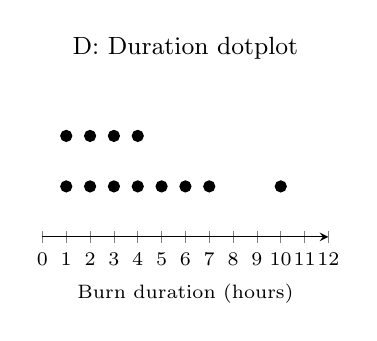
\begin{tikzpicture}\begin{axis}[width=0.43\linewidth,height=1.38in,xmin=0,xmax=12,ymin=0,ymax=3,xtick={0,1,...,12},ytick=\empty,axis y line=none,axis x line=bottom,xlabel={Burn duration (hours)},title={D: Duration dotplot},tick label style={font=\scriptsize},label style={font=\scriptsize},title style={font=\small}]
\addplot[only marks,mark=*,mark size=2pt] coordinates {(1,1) (1,2) (2,1) (2,2) (3,1) (3,2) (4,1) (4,2) (5,1) (6,1) (7,1) (10,1)};
\end{axis}\end{tikzpicture}
\end{tabular}
\end{center}
\begin{firsttakebox}{FIRST TAKE --- one sentence before you work the parts}
Which part of the proposed report needs the closest check, and why?\par
\answer{Ungraded initial position; accept a reason tied to a displayed feature.}
\end{firsttakebox}

\begin{callout}{\IconBook\ Notes on Reading Displays}{calloutgreen}
Categorical variables record labels; quantitative variables record numerical amounts with units. A distribution describes values and their frequencies. Relative frequency is count divided by total; multiply by 100 for percent.\par A bar chart compares categories. A histogram groups measurements into intervals (bins); its height counts observations in each interval. A dotplot places one dot at each recorded value, stacking repeated values. A claim about an exact value needs evidence at that precision.
\end{callout}

\dokbadge{1}~\textbf{(a)} Name the categorical variable in A and give one of its categories. Name the quantitative variable in C and its unit.\par
\answer{Wax type is categorical; Beeswax, Soy, or Paraffin is a category. Burn duration is quantitative, measured in hours.}

\dokbadge{2}~\textbf{(b)} Convert each count in A to a percent and compare with B. Explain whether these graphs represent different category distributions. \textbf{Check your response:} \fbox{\rule{0pt}{0.65em}\hspace{0.65em}} all three categories; \fbox{\rule{0pt}{0.65em}\hspace{0.65em}} total used; \fbox{\rule{0pt}{0.65em}\hspace{0.65em}} axis units.\par
\answer{Total 12. Beeswax: $6/12=50\%$; Soy: $4/12=33\frac13\%$; Paraffin: $2/12=16\frac23\%$. A and B show the same wax categories and distribution, with different vertical units. Beeswax is most common in both.}

\dokbadge{2}~\textbf{(c)} Compare what the bar from 4 to 8 in C tells you with the dots over that interval in D. State the interval count and every individual duration there, including repeats. Explain the difference in precision, using candles and hours.\par
\answer{C groups five candles into the interval from 4 hours inclusive to 8 hours exclusive. D preserves the individual durations: 4, 4, 5, 6, and 7 hours. The histogram cannot separate these exact values; the dotplot can.}

\dokbadge{3}~\textbf{(d)} $\star$ Evaluate the editor\textquotesingle s plan in a short paragraph. Defend a set of displays sufficient for both reporting questions and correct any unsupported claims using numerical evidence. The teacher scores this response E/P/I by hand; nothing is automatically scored.\par
\answer{Keep B (or A) and D for the two reporting questions. A and B show the same wax distribution: Beeswax has 6 of 12 candles, or $50\%$, so changing units does not change the most common category. C groups five candles from 4 to under 8 hours; it does not show five candles at exactly 5 hours. D shows the individual durations and only one candle at exactly 5 hours. Thus B and C alone cannot settle both questions; D supplies the required exact-value evidence.}

\begin{wordbankbox}\raggedright
\textbf{Word bank:} \textbf{individual values} \ensuremath{\;\cdot\;} C \ensuremath{\;\cdot\;} intervals \ensuremath{\;\cdot\;} \textbf{counts} \ensuremath{\;\cdot\;} category averages \ensuremath{\;\cdot\;} \textbf{D} \ensuremath{\;\cdot\;} \textbf{A} \ensuremath{\;\cdot\;} \textbf{B} \ensuremath{\;\cdot\;} \textbf{percents} \ensuremath{\;\cdot\;} cumulative totals
\par\smallskip{\footnotesize\color{framegray} bold = needed; the rest are distractors}
\end{wordbankbox}

\end{document}
